\chapter{Exploratory Data Analysis with ADI--CV Product Classification}
\section{Classification and Forecasting Prioritization of Demand Patterns }

\label{sec:adi_cv_forecasting_prioritization}

In the initial experimental phase of this study, the demand pattern classification provided by the ADI--CV framework determined which products were selected. Rather than using an additional complementary relevance-based product classifier (item) to prioritize the selected products, the analysis used only those that had been classified as \textit{smooth}. The decision to do so was based on the desire to begin evaluating forecast models on products whose demand patterns have sufficient information content (e.g., smooth), sufficient activity (i.e., non-zero values over time), and are sufficiently consistent in their behavior across all time periods.

The ADI--CV classification is particularly useful because it describes the temporal structure of each product's demand. While some products exhibit irregular, sparse, or highly variable demand, smooth products are characterized by frequent demand occurrences and comparatively stable demand sizes. These properties make them suitable as an initial benchmark subset because the forecasting errors are less likely to be dominated by excessive zero demand, extreme intermittence, or isolated demand spikes.

Therefore, the purpose of this classification stage was twofold. First, it provides a descriptive analysis of the demand behavior in the catalogue. Second, it supports the selection of a more controlled and statistically reliable subset of products for the initial forecasting experiments. In this study, the products classified as \textit{smooth} were selected as the primary benchmark subset.

\section{ADI--CV Demand-Pattern Classification}
\label{sec:adi_cv_classification}

The ADI--CV framework classifies each product according to two demand characteristics: the frequency of non-zero demand occurrences and the variability of the non-zero demand values. Let \(y_{i,t}\) denote the demand for product \(i\) at time \(t\), observed over a time horizon of length \(T_i\). The number of periods with positive demand is 

\begin{equation}
    N_i^+ = \sum_{t=1}^{T_i} \mathbb{I}(y_{i,t} > 0),
    \label{eq:non_zero_periods}
\end{equation}

where \(\mathbb{I}(\cdot)\) is an indicator function. The Average Demand Interval (ADI) is then defined as

\begin{equation}
    ADI_i = \frac{T_i}{N_i^+}.
    \label{eq:adi}
\end{equation}

The ADI measures the average number of periods between non-zero demand events. Values close to one indicate that the product sells in most of the observed periods, whereas larger values indicate more intermittent demand.

To measure the demand size variability, the coefficient of variation is computed over the non-zero demand observations. Let \(y_{i,t}^+\) denote the strictly positive demand for product \(i\). The coefficient of variation is given by the following equation:

\begin{equation}
    CV_i =
    \frac{
        \sigma(y_i^+)
    }{
        \mu(y_i^+)
    },
    \label{eq:cv}
\end{equation}

where \(\mu(y_i^+)\) and \(\sigma(y_i^+)\) denote the mean and standard deviation of nonzero demand values, respectively.

Based on these two quantities, each product is assigned to one of four demand-pattern categories:

\begin{equation}
    c_i^{ADI-CV} \in
    \{
    \text{smooth},
    \text{erratic},
    \text{intermittent},
    \text{lumpy}
    \}.
    \label{eq:adi_cv_classes}
\end{equation}


\paragraph{Smooth products.}
Smooth products exhibit regular demand and comparatively stable sales. In practical terms, these products have low ADI and CV values. Because demand is observed frequently and does not fluctuate excessively, the resulting time series are less sparse and less dominated by isolated peaks. This makes them particularly useful for evaluating whether forecasting models can capture systematic temporal behaviors.

\paragraph{Erratic products.}
Erratic products present frequent demand occurrences but have high variability in demand magnitude. In practical terms, these products have low ADI and high CV values. Although demand is observed regularly, the quantity sold fluctuates significantly over time, making the forecasting task more difficult than that for smooth products. These variations may be associated with promotions, price changes, stock availability, and other short-term demand shocks. Therefore, erratic products are relevant for later robustness analysis, but they are not selected as the first benchmark subset.

\paragraph{Intermittent products.}
Intermittent products present less frequent demand occurrences but relatively stable, nonzero demand sizes. These products are more difficult to forecast because the model must predict not only the magnitude of demand but also whether demand will occur in a given period. Their sparse nature can make error metrics difficult to interpret, especially when many periods contain zero sales.

\paragraph{Lumpy products.}
Lumpy products combine infrequent demand with high variability in demand sizes. This is the most irregular demand pattern because both the occurrence and magnitude of demand are difficult to predict. Therefore, lumpy products are not used as the first benchmark subset in this study, although they remain relevant for later robustness analysis.

\section{Dataset Distribution According to ADI--CV}
\label{sec:adi_cv_distribution}

The ADI--CV classification was applied to the complete product catalogue. The resulting distribution is presented in Table~\ref{tab:adi_cv_distribution}.

\begin{table}[H]
\centering
\caption{Distribution of products according to ADI--CV demand-pattern classification.}
\label{tab:adi_cv_distribution}
\begin{tabular}{lrr}
\hline
\textbf{Category} & \textbf{Number of items} & \textbf{Percentage} \\
\hline
Erratic & 905 & 65.1\% \\
Lumpy & 452 & 30.0\% \\
Smooth & 67 & 4.7\% \\
Intermittent & 3 & 0.2\% \\
\hline
Total & 1427 & 100.0\% \\
\hline
\end{tabular}
\end{table}

A large proportion of the catalogue (65.1\%) is classified as \emph{erratic}: these items sell frequently but with considerable variability in the quantity sold per demand occurrence. \emph{Lumpy} products form the second-largest group (30.0\%), combining infrequent demand with high size variability. The remaining two categories are comparatively rare: \emph{smooth} products account for only 4.7\% of the catalogue (67 items), while \emph{intermittent} products are rarest of all, at 0.2\% (3 items).

Smooth products exhibit the most regular and predictable demand, which makes them the cleanest setting in which to assess whether a model captures systematic temporal behaviour. On their own, however, they form too small and too homogeneous a sample to constitute a representative benchmark. The initial benchmark subset is therefore drawn from \emph{both} the smooth and erratic categories (Section~\ref{sec:smooth_erratic_product_selection}):
the two share frequent, low-ADI demand that is well suited to similarity/distance-based graph construction, while together spanning two distinct levels of forecasting difficulty, the stable smooth series and the more volatile erratic series that represent the bulk of the catalogue. Intermittent and lumpy products, whose demand is sparse and irregular, are excluded from this first stage and reserved for later robustness analysis.

\begin{figure}
    \centering
    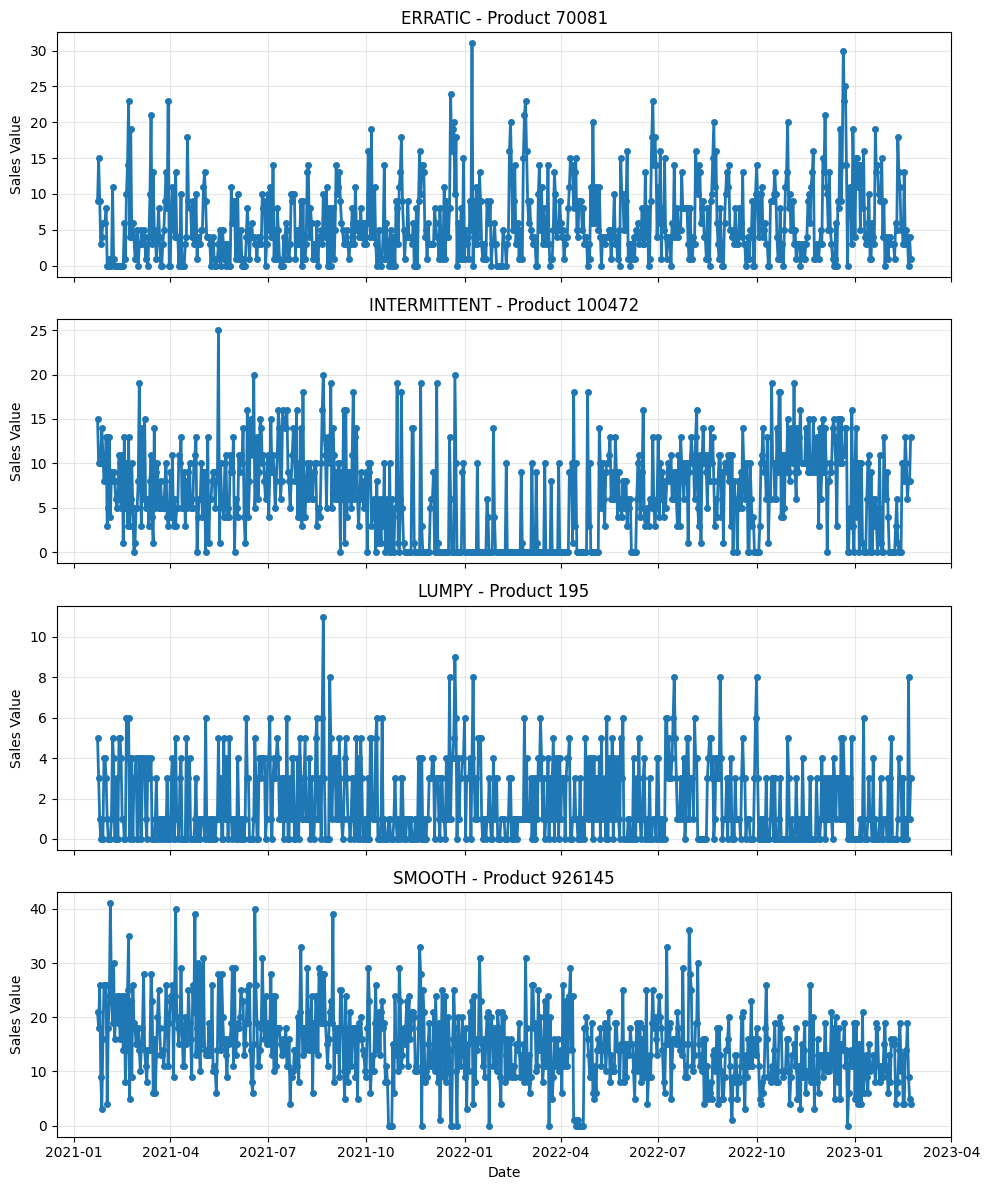
\includegraphics[width=0.5\linewidth]{figures/ADI-CV Random samples.png}
    \caption{Ilustration of samples for each ADI-CV category}
    \label{fig:placeholder}
\end{figure}
\section{Selection of Smooth and Erratic Products for the Initial Forecasting Stage}
\label{sec:smooth_erratic_product_selection}

The first experimentally-based phase is devoted to items that were identified by the ADI-CV methodology as "Smooth" or "Erratic." These product categories include items whose demands occur frequently, thereby providing a range of product demand frequency variability. This filtered data will be the base from which we construct the graphs and evaluate the models.

This choice is motivated by the objective of evaluating forecasting models for products that contain a sufficiently continuous demand signal. Both smooth and erratic products are characterized by low ADI values, indicating that demand occurs regularly across the observed period. This is important because frequent demand observations provide more informative time series data for supervised learning and reduce the risk that the evaluation is dominated by long sequences of zero sales.

Simultaneously, the inclusion of both categories allows the initial benchmark to cover two different levels of forecasting difficulty. Smooth products have relatively low demand size variability, making them more stable and easier to interpret. The forecasting performance of these products provides evidence of how well the models capture regular temporal patterns under controlled conditions.

Erratic items are characterized by a high frequency of demand occurrence, along with greater variability in the amount demanded. Because they have such high variance over time for when there is an occurrence of demand, it is harder for the model to learn as much from them as from the product type that has less volatility. However, including erratic items will provide a more accurate representation of our dataset (the entire catalog) because most of our items fall into this category.

The above selection is additionally related to the graph-based forecasting method. Graph edges are generated by the relationship (similarity/distance) of historical product time series. Therefore, it is important to select products with a sufficient history of data for effective comparison. Products with smooth histories generate consistent demand trends. Erratic products generate variable trends and determine whether relational knowledge may be useful for forecasts, even if the target series does not exhibit consistent trends.

In contrast, intermittent and lumped products were not included in the first experimental stage. These categories contain higher levels of demand sparsity, which may make forecasting errors harder to interpret and may cause similarity measures to be influenced by coincidental zero-demand periods or isolated demand spikes. Therefore, they were excluded from this analysis.



\section{Resulting Benchmark Subset}
\label{sec:resulting_benchmark_subset}
The fact that the analyzed products have adequate signals to allow the forecasting model and the construction of the similarity graph, an extra thresholding filter based on the volume of sales has been added to the ADI-CV subset. The products had to be at least at the level of minimum total world sales (i.e., each product needed to sell at least 12,500 units).

Using this filtering technique, it is possible to remove all "long tail" products. Although these are technically defined as either smooth or erratic, their very low sales volumes and consequently low levels of data density make them unreliable as inputs for our preliminary analyses. By restricting our initial analysis to this "best seller" intersection, we can assure ourselves that our models will be evaluated against a robust set of time-series in which the latent temporal structures and relationships between time-series are most clearly visible and dependable.

In the second stage, after selecting the ADI-CV pattern (smooth and erratic) for the products with respect to their demand characteristics and imposing the condition of minimum volume sales of 12,500 units, the size of the catalog of products available for evaluation was greatly reduced to a much smaller and higher signal-to-noise ratio benchmark subset. Specifically, out of the original number of 1427 products, only 60 products with smoothed and/or erratic patterns whose cumulative demand reached the minimum volume sales criterion remained in the sample. These 60 products constituted the benchmark subset of products evaluated in the first phase of the experiment.

This reduction was performed intentionally. To go from the complete catalog of 1427 products to a curated subset of 60 items, the focus of the evaluation was moved towards time series that simultaneously satisfied two requirements: frequent instances of demand occurrence (low ADI) and sufficiently large amounts of overall sales. As such, all the time series retained exhibited both sufficient temporal density and signal strength to provide both the forecasting models and the similarity-based graph construction, where edges depend on meaningful comparisons between sufficiently active demand histories.
Table~\ref{tab:benchmark_subset} summarizes the successive filtering steps that
lead to the final benchmark subset.

\begin{table}[H]
\centering
\caption{Successive filtering steps leading to the final benchmark subset.}
\label{tab:benchmark_subset}
\begin{tabular}{lr}
\hline
\textbf{Filtering step} & \textbf{Number of products} \\
\hline
Full catalogue & 1{,}427 \\
Smooth + Erratic (ADI--CV) & 972 \\
After total-sales threshold ($\geq$ 12{,}500 units) & 60 \\
\hline
\end{tabular}
\end{table}

The 60 selected products reflect both normal consumption behavior and significant sales volume. As such, they create a controlled but representative subset from which to begin; they preserve two different levels of forecasting difficulty (stable smooth products and the erratic and thus more difficult to forecast products) and allow for comparison of models without distortion due to items in the tail end of the distribution having limited historical data.

